
\documentclass[pdf]{beamer}

\usepackage{amsmath}
\usepackage{amssymb}
\usepackage{amsthm}
\usepackage{mathtools}

\usetheme{Dresden}
\usecolortheme{beaver}

%Analysis
\newcommand{\Rl}{\mathbb{R}}
\newcommand{\Cplx}{\mathbb{C}}
\newcommand{\Itgr}{\mathbb{Z}}
\newcommand{\Ntrl}{\mathbb{N}}
\newcommand{\Ind}{\mathbbm{1}}
\newcommand{\Hlbt}{\mathcal{H}}
\newcommand{\im}{\operatorname{im}}

%Algebra
\newcommand{\Grp}{\mathcal{G}}

%Misc
\newcommand{\lra}{\longrightarrow}
\newcommand{\ra}{\rightarrow}
\newcommand{\lla}{\longleftarrow}
\newcommand{\la}{\leftarrow}

%Stats \ Prob
\newcommand{\E}[1]{\mathbb{E} \left[ #1 \right]}
\newcommand{\Var}[1]{\operatorname{Var} \left[ #1 \right] }
\newcommand{\Cov}[2]{\operatorname{Cov} \left[ #1, #2 \right] }
\newcommand{\Filt}{\mathcal{F}}

%Fractional Differential Equations

\newcommand{\laplace}[1]{ \mathcal{L} \left\{ #1 \right\} }
\newcommand{\fourier}[1]{ \mathcal{F} \left\{ #1 \right\} }
\newcommand{\mellin}[1]{ \mathcal{M} \left\{ #1 \right\} }
\newcommand{\rld}[3]{ \left( \mathcal{D}_{#1}^{#2} #3 \right) }
\newcommand{\rli}[3]{ \left( I_{#1}^{#2} #3 \right) }
\newcommand{\der}[3]{ \frac{d^{#3}#1}{d#2^{#3}} }
\newcommand{\capder}[3]{ \left( \prescript{C}{}{\mathcal{D}_{#1}^{#2}} #3 \right) }

\mode<presentation>{}
\title{A Stochastic Approach to Fractional Diffusion}
\subtitle{help I'm trapped in a LaTeX compiler}
\author{Ed McDonald \& Adam Gray}
\institute{
	School of Mathematics and Statistics \\
	University of New South Wales
}

\begin{document}

\begin{frame}
	\titlepage
\end{frame}

\begin{frame}{Outline}
    \begin{itemize}
        \item Derivation of Standard Diffusion
        \item Derivation of Super Diffusion
        \item Time Fractional Diffusion
        \item Applications
    \end{itemize}
\end{frame}


\begin{frame}{Central Limit Theorem and Random Walks}
	\begin{block}{Random Walk}
	    Let $ X_1, \ldots X_n $ be a sequence of random variables,
	    then 
	    \begin{align}
	        S_n = \sum_{k=1}^n X_n 
	    \end{align}
	    represents the position after $ n $ steps.
	\end{block}
	If $ \mathbb{E}[X_i] = 0 $ and  $ \mathbb{E}[X_i^2] = 2 $ then the central limit theorem gives us that
	\begin{align}
	    \frac{S_n}{\sqrt{n}} \lra Z
	\end{align}
	\emph{weakly} as $ n \lra \infty $, where $ Z \sim \mathcal{N}(0,2) $
\end{frame}

\begin{frame}{Central Limit Theorem and Random Walks}
    We can extend this idea by introducing a scaling parameter $ \gamma $.
    \begin{align}
        S_{\lfloor \gamma t \rfloor} = \sum_{k=1}^{\lfloor \gamma t \rfloor} X_k.
    \end{align}
    $ \gamma $ has the effect of changing the \emph{timescale} that we are considering the process running over.
    
    We can calculate the characteristic function of 
    \begin{align}
       \frac{S_{\lfloor \gamma t \rfloor}}{\sqrt{\gamma }}.
    \end{align}
    By the convolution theorems we can say that it is
    \begin{align}
        \left( 1- \frac{k^2}{\gamma} + o(\gamma^{-1}) \right)^{\lfloor \gamma t \rfloor}
    \end{align}
\end{frame}

\begin{frame}{Long Time Limit}
    We can rearrange
    \begin{align}
        \left( 1- \frac{k^2}{\gamma} + o(\gamma^{-1}) \right)^{\lfloor \gamma t \rfloor}
        &= \left[ \left( 1- \frac{k^2}{\gamma} + o(\gamma^{-1}) \right)^\gamma \right]^\frac{{\lfloor \gamma t \rfloor}}{\gamma}
    \end{align}
    and then take $ \gamma \lra \infty $ to get that
    \begin{align}
    \left[ \underbrace{\left( 1- \frac{k^2}{\gamma} + o(\gamma^{-1}) \right)^\gamma}_{\circledast} \right]^\frac{{\lfloor \gamma t \rfloor}}{\gamma} \lra e^{-tk^2}
    \end{align}
    by using the well known result
    \begin{align}
        \lim_{n \lra \infty} \left(1 + \frac{x}{n}\right)^n = e^x.
    \end{align}
\end{frame}


\begin{frame}{Fourier Transform and a PDE}
    Notice that $ e^{-tk^2} $ is just the CF of $Z_t \sim \mathcal{N}(0,2t) $. Further we can say that $ \frac{S_{\lfloor \gamma t \rfloor}}{\sqrt{\gamma}} \lra Z_t $ by LCT.
    
    
    We can also regard $ e^{-tk^2} $ as the FT of the density of $ Z_t $.
    
    Rather usefully we have also have that $ e^{-tk^2} $ is a solution to 
    \begin{align}
        \frac{d\hat{u}}{dt} = -k^2\hat{u}
    \end{align}
    
    We can actually use a analogous result from last week's homework to invert the Fourier transform of $ u $ to get
    \begin{align}
        \frac{\partial u}{dt} = \frac{\partial^2 u}{\partial x^2}
    \end{align}
\end{frame}

\begin{frame}{A More General Result}
    We can generalize this result a bit and say that if $ \mathbb{E}[X_i^2] = \sigma^2 $
    then $ \frac{S_{\lfloor \gamma t \rfloor}}{\sqrt{\gamma}} \lra Z_{t} $, but now $ Z_t \sim \mathcal{N}(0,2\sigma^2 t) $.
    
    Further the Fourier transform of the density of $ Z_t $ is $ e^{-t\sigma^2k^2} $
    which means the density is now a solution to
    \begin{align}
        \frac{\partial u}{\partial t} = \underbrace{\frac{\sigma^2}{2}}_{D}\frac{\partial^2 u}{\partial x^2}.
    \end{align}
    What this says is that as particles jump around more, they diffuse more rapidly.
\end{frame}


\begin{frame}{A Plot}
    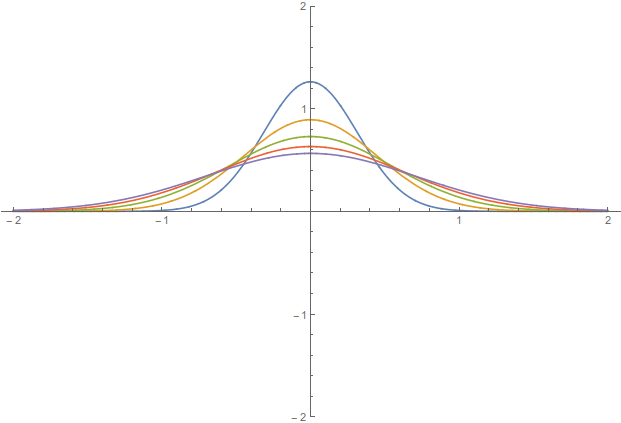
\includegraphics[scale=0.4]{Diffusion}
\end{frame}

\begin{frame}{Recap}
    \begin{itemize}
        \item All we have done to get this result is require that the random variables that represent the \emph{jumps} fulfill the requirements of the CLT.
        \item What if we relax the \emph{finite second moment} condition?
    \end{itemize}
\end{frame}
\begin{frame}{Pareto Distribution}
    \begin{itemize}
        \item Consider a random variable $ P $ with density $ Cx^{-\alpha-1} $ for some normalizing constant $ C $.
        \item If we require $ 1 < \alpha < 2 $ then we have $ \mathbb{E}[P] $ exists but $ \mathbb{E}[P^2] = \infty $ does not.
        \item It can be shown (with very lengthy computation) that the FT of the density of $ P $ is $ 1 + (ik)^\alpha + O(k^2) $.
        \item The idea is to setup a sequence of random variables $ Y_1, \ldots Y_n $, all iid with Pareto distribution with parameter $ \alpha $ and use these as the \emph{jumps} in the random walk.
    \end{itemize}
    
\end{frame}

\begin{frame}{Pareto Distribution}
    Setup $ S_n = \sum_{k=1}^n Y_n $ as before.
    
    By the convolution theorems for FTs we can calculate the FT of the density of $ \frac{S_n}{n^\frac{1}{\alpha}} $ to be
    \begin{align}
        \left( 1 + \frac{(ik)^\alpha}{n} + O(n^{-\frac{2}{\alpha}}) \right)^n
    \end{align}
    Notice that as $ n \lra \infty $ this has limit $ e^{(ik)^\alpha} $.
    
    The LCT implies that $ \frac{S_n}{n^\frac{1}{\alpha}} \lra Z $ where $ Z $ has FT $ e^{(ik)^\alpha} $.
    
    Notice that in some way this is an \emph{Extended Central Limit Theorem}.
\end{frame}

\begin{frame}{Long Time Limit}
    Like before we can introduce a time scale parameter $ \gamma $ and write
    \begin{align}
        S_{\lfloor \gamma t \rfloor} = \sum_{k=1}^{\lfloor \gamma t \rfloor}Y_k.
    \end{align}
    Again by considering the FT of 
    \begin{align}
        \frac{S_{\lfloor \gamma t \rfloor}}{\gamma^\frac{1}{\alpha}}
    \end{align}
    which is
    \begin{align}
        \left( 1 + \frac{(ik)^\alpha}{\gamma} + o(\gamma^\frac{-2}{\alpha})\right)^{\lfloor \gamma t \rfloor}.
    \end{align}
\end{frame}

\begin{frame}{Long Time Limit}
    \begin{align}
            \left( 1 + \frac{(ik)^\alpha}{\gamma} + o(\gamma^\frac{-2}{\alpha})\right)^{\lfloor \gamma t \rfloor}
        \end{align}
        By taking $ \gamma \lra \infty $ we get that the Fourier transform converges to
        \begin{align}
            e^{t(ik)^\alpha}
        \end{align}
    and by the LCT this gives us that 
    \begin{align}
        \frac{S_{\lfloor \gamma t \rfloor}}{\gamma^\frac{1}{\alpha}} \lra Z_t
    \end{align}
    where $ Z_t $ has FT $ \hat{u}(k) = e^{t(ik)^\alpha} $.
    
    Notice that this is a stable distribution.
\end{frame}
\begin{frame}
    It is clear that $ \hat{u}(t) = e^{t(ik)^\alpha} $ is a solution to
    \begin{align}
        \frac{d\hat{u}}{dt} = (ik)^\alpha \hat{u}.
    \end{align}
    Unfortunately we can't use \emph{last week's homework} to invert this FT and this is where we introduce fractional calculus.
\end{frame}


\begin{frame}{Motivations}
	\begin{block}{Cauchy Formula for Repeated Integration}
		\begin{align*}
			\int_{a}^{x} \int_{a}^{y_1} \cdots \int_a^{y_{n-1}} f(y_n) dy_n \cdots dy_2 dy_1 = \frac{1}{(n-1)!} \int_a^x(x-t)^{n-1}f(t)dt
		\end{align*}
	\end{block}
	\pause
	The idea is to replace the factorials with gamma functions to define an integral of arbitrary order
	\pause
	\begin{block}{Riemann-Liouville Fractional Integral}
		\begin{align*}
			\rli{a}{\alpha}{f}(x) = \frac{1}{\Gamma(\alpha)} \int_a^x(x-t)^{\alpha-1}f(t)dt
		\end{align*}
	\end{block}
\end{frame}

\begin{frame}{Motivations (Derivatives)}
	\begin{block}{Riemann-Liouville Fractional Derivative}
		\begin{align*}
			\rld{a}{\alpha}{f}(x) &= \frac{d^{\lceil \alpha \rceil}}{dx^{\lceil \alpha \rceil}} \rli{a}{\lceil \alpha \rceil - \alpha}{f}(x) \\
				&= \frac{1}{\Gamma(1 - \alpha)}\frac{d^{n}}{dx^n} \int_a^x \frac{f(t)dt}{(x-t)^{\alpha - n + 1}}
		\end{align*}
		where $ n = \lfloor \alpha \rfloor + 1 $.
	\end{block}
\end{frame}

\begin{frame}{Motivations (Derivatives)}
	\begin{block}{Caputo Fractional Derivative}
		\begin{align*}
			\capder{a}{\alpha}{f}(x) &= \rli{a}{\lceil \alpha \rceil - \alpha}{\frac{d^{\lceil \alpha \rceil}}{dx^{\lceil \alpha \rceil}}f}(x) \\
				&= \frac{1}{\Gamma(1 - \alpha)} \int_a^x \frac{\frac{d^{t}}{dt^n}f(t)dt}{(x-t)^{\alpha - n + 1}}
		\end{align*}
		where $ n = \lfloor \alpha \rfloor + 1 $.
	\end{block}
\end{frame}
\begin{frame}{ Riemann-Liouville vs Caputo Derivative}
    \begin{itemize}
	\item The Caputo derivative is often used in fractional differential equations because it
	can be coupled with integer order initial conditions, whereas often the Riemann-Liouville
	derivative can't be coupled with integer order initial conditions.
   
    \item When we set $ a = -\infty $ for a large class of functions these derivatives are the same.
    \end{itemize}
\end{frame}

\begin{frame}{Fractional Derivative Fourier Transform}

	It can be shown that
	\begin{align}
	    \mathcal{F}\left\{\prescript{}{-\infty}{\mathcal{D}^\alpha}f(x) \right\} = (ik)^\alpha \mathcal{F}\{ f(x) \}
    \end{align}
    and it is precisely this result that we use to \emph{invert} the Fourier transform we had before.
    That is we can say that
    \begin{align}
        \frac{\partial u}{\partial t}(x,t) = \prescript{}{-\infty}{\mathcal{D}^\alpha_x} u(x,t)
    \end{align}
    where $u $ is the density of $ Z_t = \lim_{\gamma\lra\infty} \frac{Y_1 + Y_2 + \cdots + Y_{\lfloor \gamma t \rfloor}}{\gamma^\frac{1}{\alpha}} $.
    
    It can be shown that $ u(x,t) = Ax^{-\alpha-1} + o(x^{-\alpha-1}) $ as $ x \lra \infty $ with $ A $ depending on $ t $ and $ \alpha $.
\end{frame}

\begin{frame}{Fractional Derivative Fourier Transform}

    Actually this isn't entirely the case...
    In space we will often use a \emph{Riesz} or \emph{Riesz-Feller} fractional derivative. 
    
    The Riesz fractional derivative of a function $ f $ is defined as 
    \begin{align}
        \mathcal{F}^{-1}\{-|k|^\alpha \hat{f}(k) \}(x).
    \end{align}
    The reason one does this is because $ e^{(ik)^\alpha} $ isn't really well defined for non-integer $ \alpha $ and $ k < 0 $. 
\end{frame}

\begin{frame}{Time Fractional Diffusion}
    \begin{itemize}
        \item A similar idea can be applied to the \emph{time} between steps. 
        \item This is done by considering something called a continuous time random walk.
        \item If we choose the distribution to be the \emph{exponential} distribution we get get normal diffusion.
        \item If we choose something different, say the \emph{Mittag-Leffler} distribution, then we can get time-fractional diffusion.
        \item This is where the time derivative is fractional.
    \end{itemize}
\end{frame}
	

\begin{frame}{Coupled Continuous Time Random Walks}
    \begin{itemize}
        \item One can go even further with space and time derivatives. 
        \item If we assume that the waiting times between jumps and time size of the jumps are independent then we get a \emph{decoupled} random walk.
        \item If we don't assume this then we get a coupled random walk. This has particularly interesting applications in finance.
    \end{itemize}
\end{frame}

\begin{frame}{Applications}
    \textbf{Finance}
    \begin{itemize}
        \item Raberto, M., Scalas, E., Gorenflo, R., \& Mainardi, F. (2000). The waiting-time distribution of LIFFE bond futures. arXiv preprint cond-mat/0012497
        \item Scalas, E., Gorenflo, R., \& Mainardi, F. (2000). Fractional calculus and continuous-time finance. Physica A: Statistical Mechanics and its Applications, 284(1), 376-384.
    \end{itemize}
    \textbf{Biology}
    \begin{itemize}
        \item Goychuk, I., \& Hänggi, P. (2004). Fractional diffusion modeling of ion channel gating. Physical Review E, 70(5), 051915.
    \end{itemize}
    \textbf{Chemistry}
    \begin{itemize}
        \item Bazelyansky, M., Robey, E., \& Kirsch, J. F. (1986). Fractional diffusion-limited component of reactions catalyzed by acetylcholinesterase. Biochemistry, 25(1), 125-130.
    \end{itemize}
\end{frame}

\begin{frame}{Acknowledgement}
    This talk was partly based off ideas outlined in
    
    Meerschaert, M. M., \& Sikorskii, A. (2011). Stochastic models for fractional calculus (Vol. 43). Walter de Gruyter.
\end{frame}

\end{document}
